\begin{tikzpicture}[x=1cm,y=1cm,font=\small]
  \useasboundingbox (-0.15,-2.05) rectangle (14.1,3.5);
  \begin{scope}
    \node[align=center] at (2.05,3.1) {(a) Mutable point and\\residual intersections};
    \draw[thick] (0,1.25)--(4.05,1.25);
    \node[above left] at (0,1.25) {$D_E$};
    \foreach \position in {2.7,3.65} {
      \draw[blue!70!black,thick] (\position-0.15,0.65)--(\position+0.15,1.85);
      \fill[blue!70!black] (\position,1.25) circle (2.5pt);
    }
    \fill[orange!65!black] (1.05,1.25) circle (3pt);
    \node[below,align=center] at (1.05,1.05) {$p_E$\\$x=-1$};
    \node[text=blue!70!black,align=center] at (3.15,2.2) {simple residual\\roots};
    \node at (2.05,-0.55) {$(1+x)^{m\ell}r_E(x)$};
    \node at (2.05,-1.15) {$r_E(-1)\ne0$};
  \end{scope}
  \begin{scope}[xshift=4.9cm]
    \node[align=center] at (2,3.1) {(b) Weighted Newton\\segment};
    \draw[->] (0.35,0.2)--(3.85,0.2) node[right] {$t$};
    \draw[->] (0.35,0.2)--(0.35,2.55) node[above] {$u$};
    \draw[orange!65!black,thick] (0.35,2.1)--(3.25,0.2);
    \fill[orange!65!black] (0.35,2.1) circle (2pt);
    \fill[orange!65!black] (3.25,0.2) circle (2pt);
    \node[above right] at (0.35,2.1) {$(0,\ell)$};
    \node[below] at (3.25,0.15) {$(m\ell,0)$};
    \node at (2,-0.55) {$\operatorname{wt}(t)=1,\quad\operatorname{wt}(u)=m$};
    \node at (2,-1.25) {$F_0=t^{m\ell}Q\!\left(\dfrac{u}{t^m}\right)$};
  \end{scope}
  \begin{scope}[xshift=9.8cm]
    \node[align=center] at (2,3.1) {(c) Smooth branches\\with contact $m$};
    \draw[gray!70,->] (0.15,0.35)--(3.85,0.35) node[right] {$t$};
    \draw[gray!70,->] (2,0.05)--(2,2.15);
    \node[gray!70,anchor=west] at (2.05,1.75) {$u$};
    \foreach \coefficient in {0.3,0.6,0.9}
      \draw[orange!65!black,thick,domain=-1.4:1.4,samples=45]
        plot ({2+\x},{0.35+\coefficient*\x*\x});
    \fill[orange!65!black] (2,0.35) circle (2.5pt);
    \node[text=orange!65!black] at (2,2.4) {$\ell$ branches};
    \node at (2,-0.35) {$u=\alpha_jt^m+\cdots$};
    \node at (2,-0.9) {$I(C_i,C_j)=m$};
    \node[align=center] at (2,-1.65)
      {$\delta_E=\sum_{i<j}I(C_i,C_j)$\\[3pt]$=m\binom{\ell}{2}$};
  \end{scope}
\end{tikzpicture}